%!TEX root = ../vortrag.tex
\section{Funktionale Programmierung}
\begin{frame}[t]{Funktionale Programmierung} \label{folie:funktional}
	\begin{center} \small
		\textit{\enquote{Jedes berechenbare Problem kann auf die Auswertung einer Funktion reduziert werden.}} \ccite{info1}{}
	\end{center}
	\textbf{Merkmale der funktionalen Programmierung:}
	\begin{itemize}
		\item Ausführung eines Programms entspricht Auswertung einer Funktion. 
		\item Variablen sind Bezeichner, deren Werte während der Auswertung konstant bleiben \bet{(Zustandslosigkeit)}
		\begin{itemize}
			\item Insbesondere: Eine Variable kann durch den korrespondierenden Wert ersetzt werden, ohne das Verhalten des Programms zu verändern \bet{(Referenzielle Transparenz)}
		\end{itemize}
		\item Prozeduren als \bet{Daten erster Klasse}.
		\item Theoretische Grundlage: Lambda-Kalkül.
	\end{itemize}
\end{frame}

\begin{frame}[t,fragile]{Scheme und Racket}
	\begin{minipage}{0.6\textwidth}
	\begin{itemize}
		\item In diesem Vortrag verwendet: Scheme-Sprachstandard R\textsuperscript{5}RS (1998)
		\item Verwendbar in DrRacket 7.0 mittels Direktive \mintinline{scheme}{#lang r5rs}.
		\item \textit{Racket Teaching Languages} weitestgehend kompatibel mit R\textsuperscript{5}RS (Sprachstufe: \textit{Advanced Student} oder \textit{Intermediate Student with lambda})
		\item ggfs. unterschiedliche (bzw. unterschiedlich genaue) Rückgaben des Interpreters.
	\end{itemize}
	\end{minipage}~\hfill~
	\begin{minipage}{0.3\textwidth}
		\includegraphics[keepaspectratio,width=4cm]{img/racket-logo.pdf}
	\end{minipage}
	
\end{frame}

\begin{frame}[t,fragile]{Zusammengesetzte Ausdrücke}
	\begin{itemize}
		\item Zusammengesetzte Ausdrücke in geklammerter Präfix-Notation:
		\begin{center}
			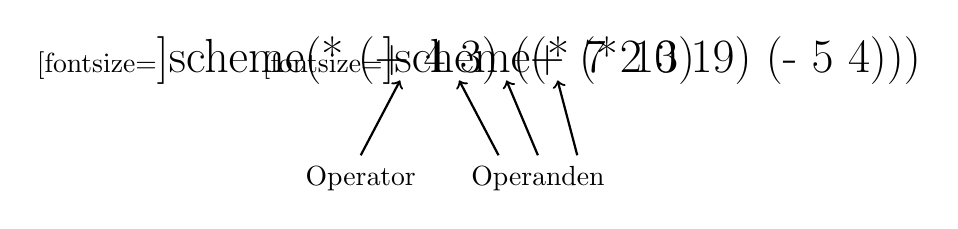
\begin{tikzpicture}
				%\draw [step=0.5cm] (-2,-1) grid (2,1);
				\draw<1|handout:0> (0,0) node{\mintinline[fontsize=\LARGE]{scheme}{(* 7 2 3)}};
				\onslide<1|handout:0>{
				\draw (-1.5,-1.5) node{Operator};
				\draw (0.75,-1.5) node{Operanden};
				\draw [->,thick] (-1.5,-1.2) -- (-1,-0.25);
				\draw [->,thick] (0.25,-1.2) -- (-0.25,-0.25);
				\draw [->,thick] (0.75,-1.2) -- (0.35,-0.25);
				\draw [->,thick] (1.25,-1.2) -- (1,-0.25); }
				\draw<2-> (0,0) node{\mintinline[fontsize=\LARGE]{scheme}{(* (+ 4 3) (+ (* 10 19) (- 5 4)))}};
			\end{tikzpicture}
		\end{center}
	\end{itemize}
	\onslide<3->{
	\begin{mybox}
		Auswertung des zusammengesetzten Ausdrucks $\mathtt{(op \ exp_1 \ exp_2 \ \dots \ exp_k)}$: \\ \ccite{sicp}{Kap. 1.1.3}
		\begin{enumerate}[(1)]
			\item<4-> Werte die Teilausdrücke $\mathtt{op}, \mathtt{exp_1}, \mathtt{exp_2}, \dots, \mathtt{exp_k}$ aus.
			\item<5-> Wende die Auswertung von $\mathtt{op}$ auf die Auswertungen von $\mathtt{exp_1}, \dots, \mathtt{exp_k}$ an.
		\end{enumerate}
	\end{mybox}}
	\begin{itemize}
	\item<6->[$\Rightarrow$] Rekursives Auswertungsprinzip. 
	\end{itemize}
\end{frame}

\begin{frame}[t,fragile]{}
	\bet{Beispiel:} Auswertung von \mintinline{scheme}{(* (+ 4 3) (+ (* 10 19) (- 5 4)))}
	
	\begin{center}
	\begin{tikzpicture}[level 1/.style = {sibling distance=4cm},
	    level 2/.style = {sibling distance=2cm}, 
	    level 3/.style = {sibling distance=1cm}, 
	    level distance = 1cm,
		every node/.style = {shape=circle,font=\ttfamily,
	    draw=maincolor,thick, align=center,
	    top color=white, bottom color=white}]]
	  \onslide<2|handout:2>{
		  \node {*}
		    child { node {+}
		    	child { node {4} }
		    	child { node {3} } }
		    child { node {+}
		      child { node {*}
		        child { node {10} }
		        child { node {19} }}
		      child { node {-}
		        child { node {5} }
		        child { node {4} }}};	}
	  \onslide<3|handout:3>{
		  \node {*}
		    child { node {7}}
		    child { node {+}
		      child { node {190}}
		      child { node {1}}};	}
	  \onslide<4|handout:4>{
	  	\node {*}
    		child { node {7}}
		    child { node {191}};	}
	  \onslide<5|handout:5>{
	  	\node {1337};	}		      
	\end{tikzpicture}
	
	\vspace*{0.5cm}
	
	\ttfamily
	\begin{tabular}{l}
		\onslide<2-|handout:2->{(* (+ 4 3) (+ (* 10 19) (- 5 4)))} \\[0.25cm]
		\onslide<3-|handout:3->{$\rightarrow$ (* 7 (+ 190 1))}                   \\[0.25cm]
		\onslide<4-|handout:4->{$\rightarrow$ (* 7 191)}                         \\[0.25cm]
		\onslide<5-|handout:5->{$\rightarrow$ 1337}
	\end{tabular} 
	
	\end{center}
\end{frame}

\begin{frame}[t,fragile]{}
	\begin{mybox}
		Auswertung eines zusammengesetzten Ausdrucks $\mathtt{(op \ exp_1 \ exp_2 \ \dots \ exp_k)}$:
		\begin{enumerate}[(1)]
			\item Werte die Teilausdrücke $\mathtt{op}, \mathtt{exp_1}, \mathtt{exp_2}, \dots, \mathtt{exp_k}$ aus.
			\item Wende die Auswertung von $\mathtt{op}$ auf die Auswertungen von $\mathtt{exp_1}, \dots, \mathtt{exp_k}$ an.
		\end{enumerate}
	\end{mybox} \pause
	
	\vspace*{0.5cm}
	
	\bet{Fragen:}
	\begin{itemize}
		\item In welcher Reihenfolge werden die $\mathtt{exp_i}$ und $\mathtt{op}$ ausgewertet? \pause
		\begin{itemize}
			\item \enquote{[\dots] the order of evaluation is unspecified, and the operator expression and the operand expressions are always evaluated with the same evaluation rules.} \ccite{r5rs}{Kap. 4.1.3}
			\item[$\Rightarrow$] Compiler-/Interpreterabhängiges Verhalten.
			\item Racket: Auswertung von links nach rechts \ccite{racket}{Kap. 4.3.1}
		\end{itemize}
		\item Warum muss $\mathtt{op}$ ebenfalls ausgewertet werden? \pause
		\begin{itemize}
			\item $\mathtt{op}$ kann ebenfalls ein zusammengesetzter Ausdruck sein.
		\end{itemize}
		\item Was passiert bei der Auswertung von $\mathtt{op}$?
		\begin{itemize}
			\item Bisher nur elementare \minor{(= eingebaute)} Prozeduren gesehen.
		\end{itemize}
	\end{itemize}
\end{frame}